\begin{figure}
    \centering
    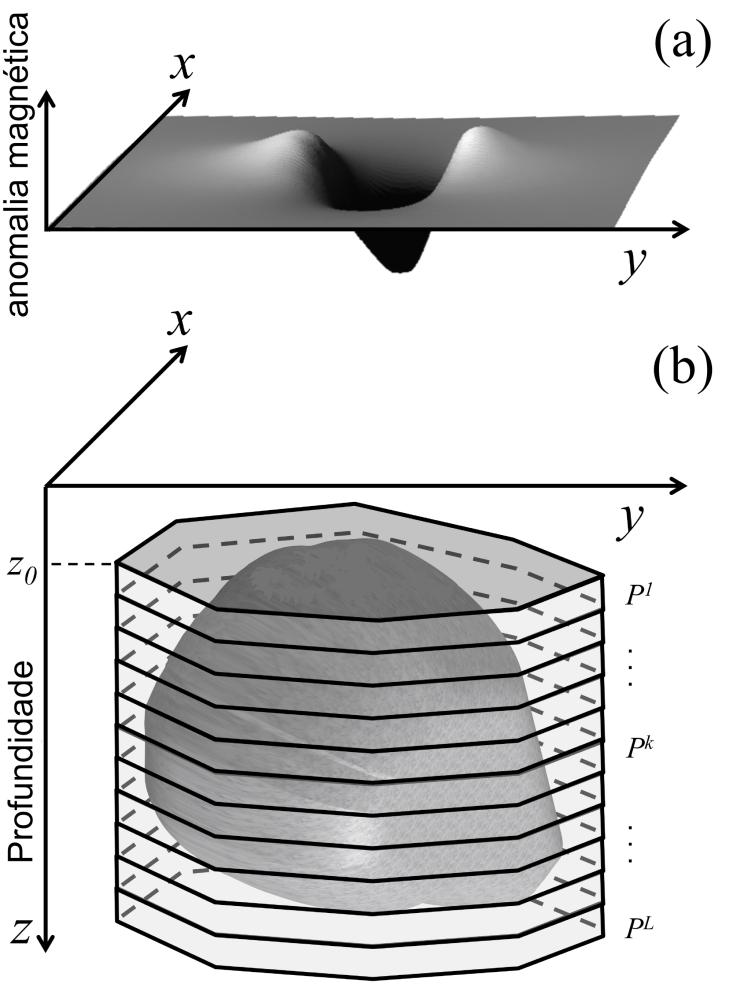
\includegraphics[scale=0.3]{figures/observed_data.png}
    \caption{Schematic representation of (a) total-filed anomaly (grey surface) produced by (b) a 3-D anomalous source (dark grey volume). The interpretation model in (b) consists of a set of L vertical, juxtaposed 3-D prisms $P^k$ , $k = 1,\dots, L$, (light grey prisms) in the vertical direction of a right-handed coordinate system.}
    \label{fig:obs}
\end{figure}

\begin{figure}
    \centering
    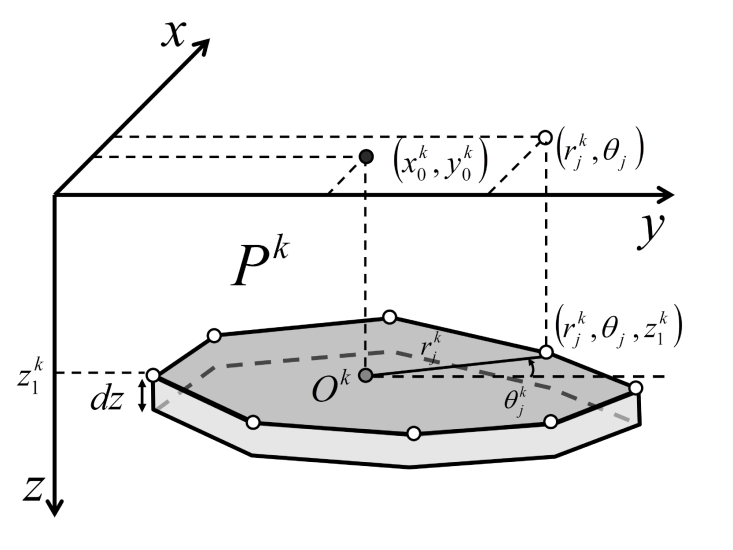
\includegraphics[scale=0.3]{figures/prism_parameters_mod.png}
    \caption{Polygonal cross-section of the $k$th vertical prism $P^k$ described by $V$ vertices (white dots) with polar coordinates ($r^k_j$ , $\theta ^k_j$), $j = 1, \dots, V$, $k = 1, \dots, L$ , referred to an arbitrary origin $O^k$ (grey dot) with horizontal Cartesian coordinates ($x_0^k$ , $y_0^k$), $k = 1, \dots, L$ , (black dot).}
    \label{fig:prism_parameters}
\end{figure}

\begin{figure}
    \centering
    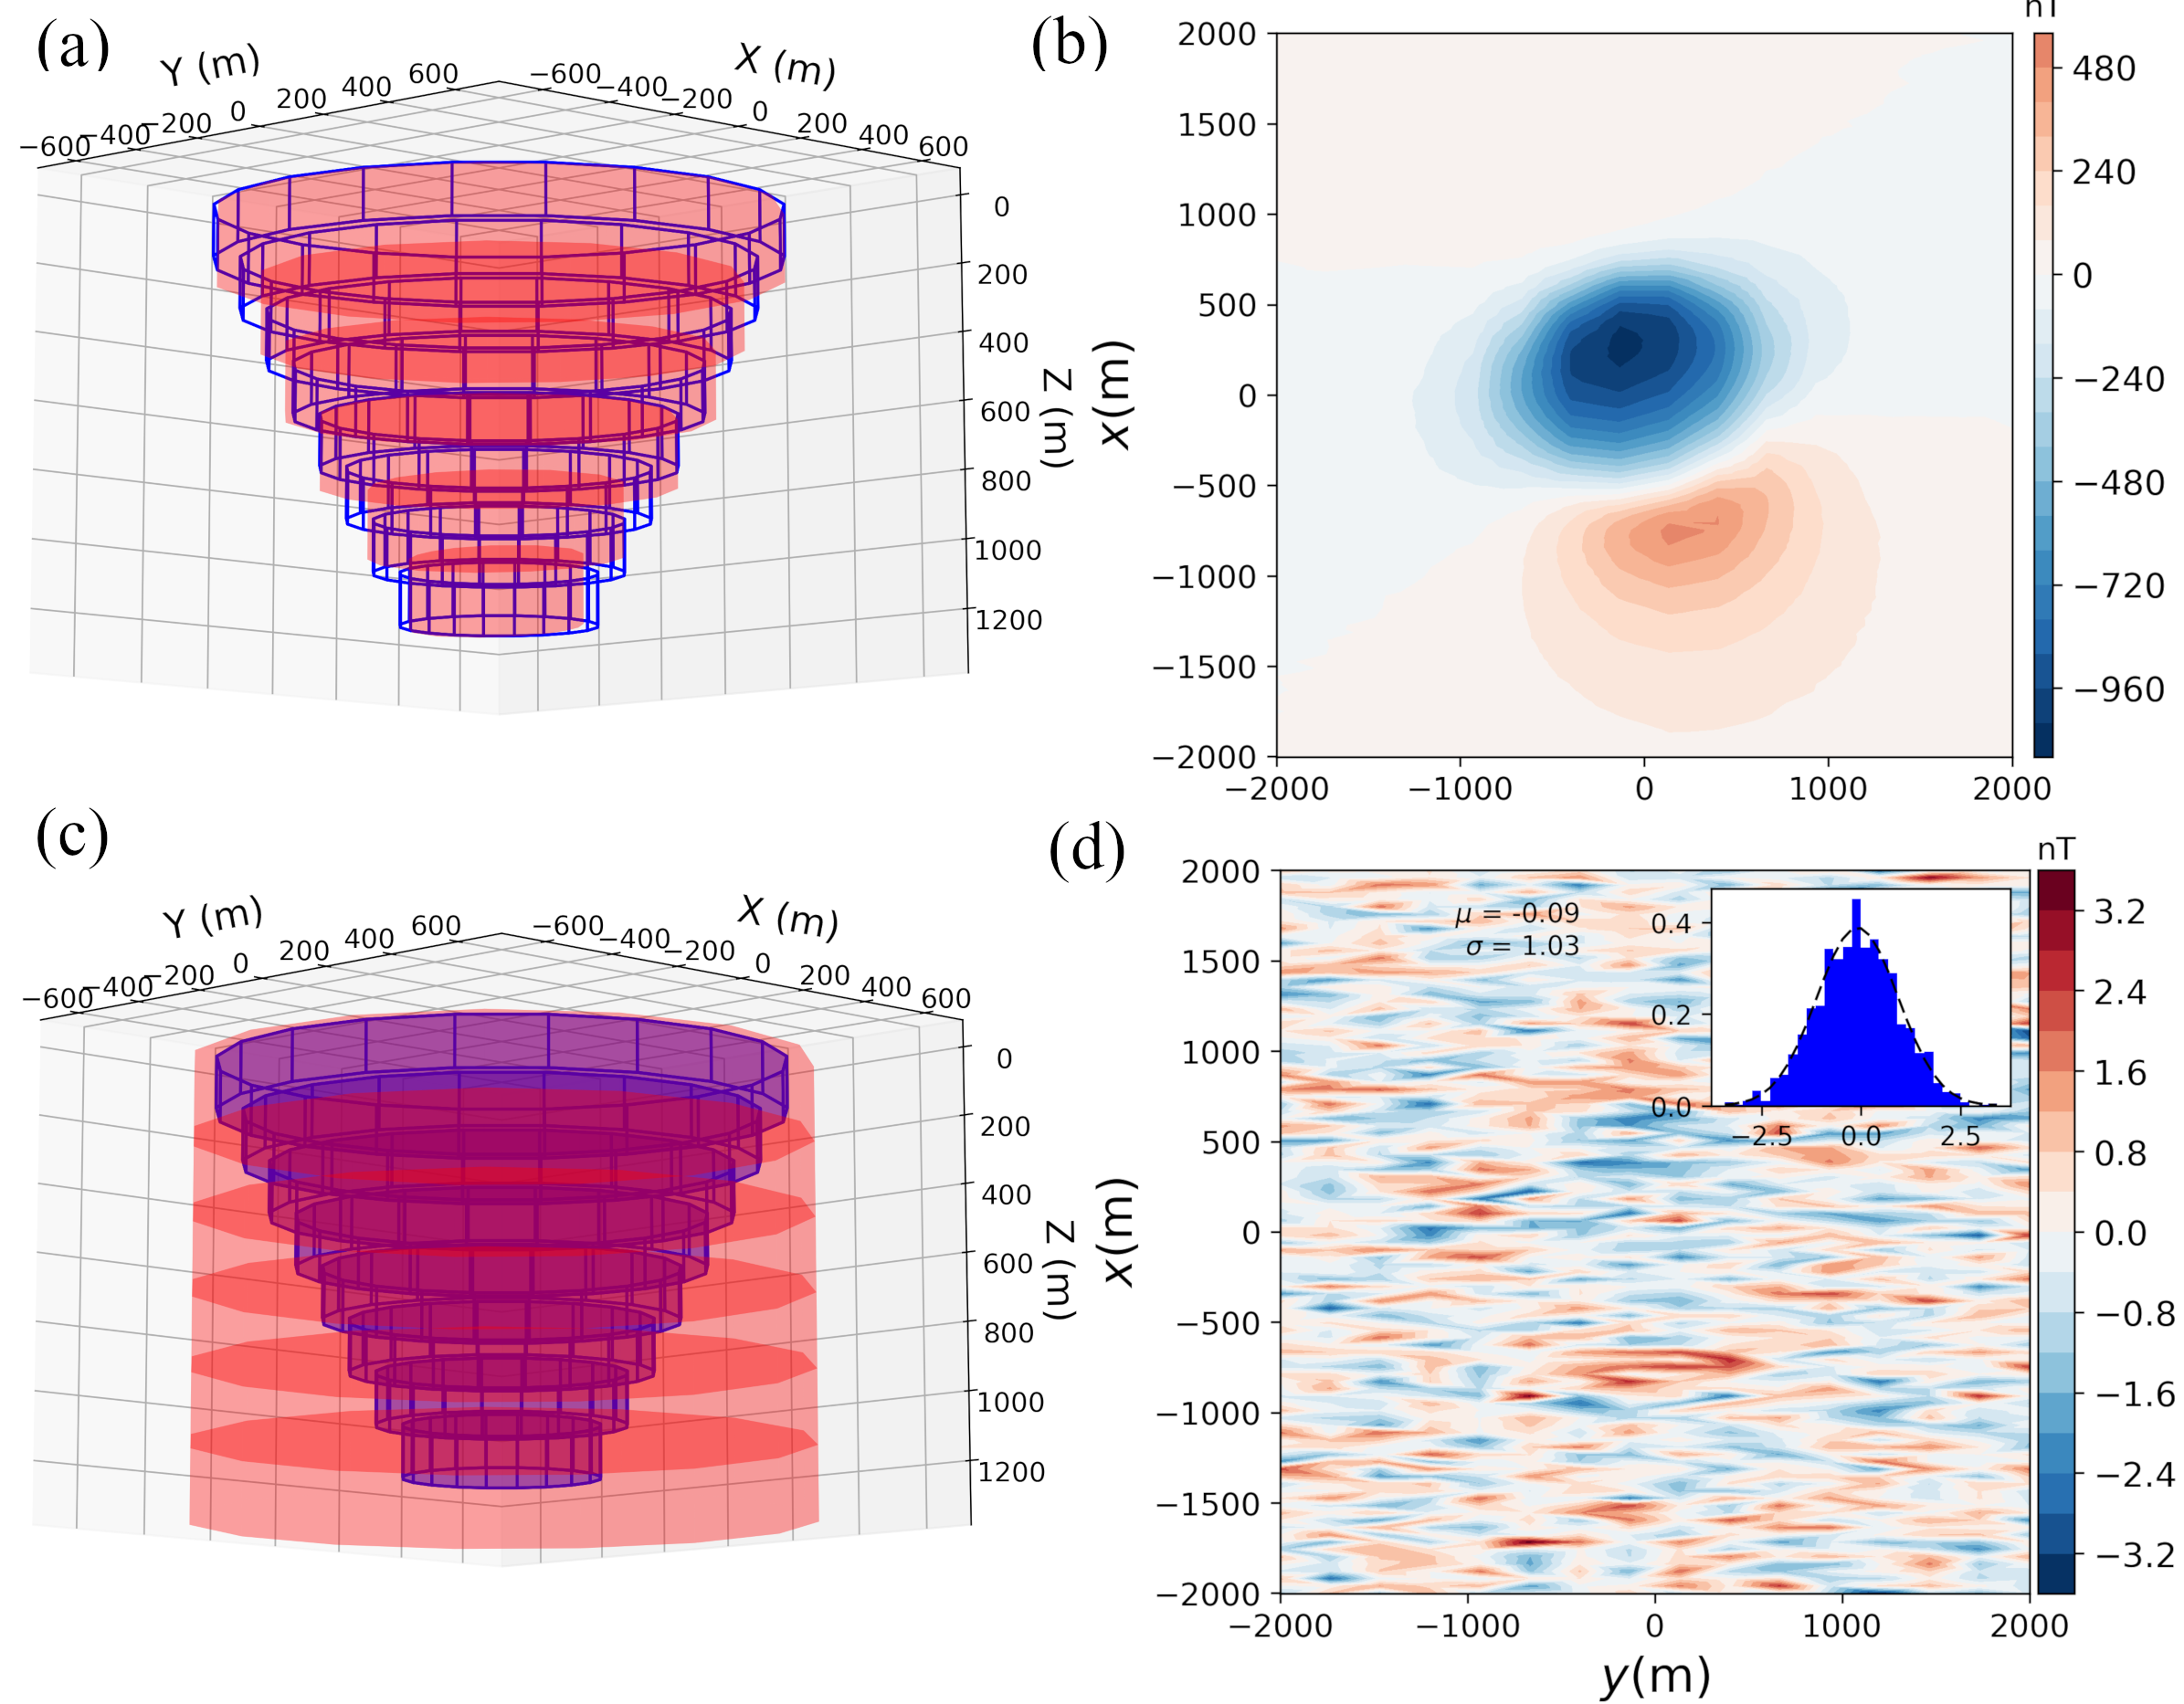
\includegraphics[scale=.75]{figures/kimberlite_4figures.png}
    \caption{(a) Perspective view of the simple model with the depth to the top $z_0 = 50$ m and the depth extent $1200$ m. (b) Synthetic noise-corrupted total-field anomaly produced by the simple model blue prisms in (a). The data was contaminated by a pseudorandom Gaussian noise with mean zero and standard deviation $1$ nT. (c) Perspective view of the true (blue lines) and estimated body (red prisms) obtained by inverting the noise-corrupted total-field anomaly in (b). (d) Residuals defined as the difference between the noisy and the predicted (not shown) total-field anomalies; the latter was produced by the estimated body (red prisms in b). The inset in d shows the histogram and the Gaussian curve for the residuals with mean $\mu=0.1$ nT and standard deviation $\sigma=5.23$ nT.
}
    \label{fig:kimb}
\end{figure}

\begin{figure}
    \centering
    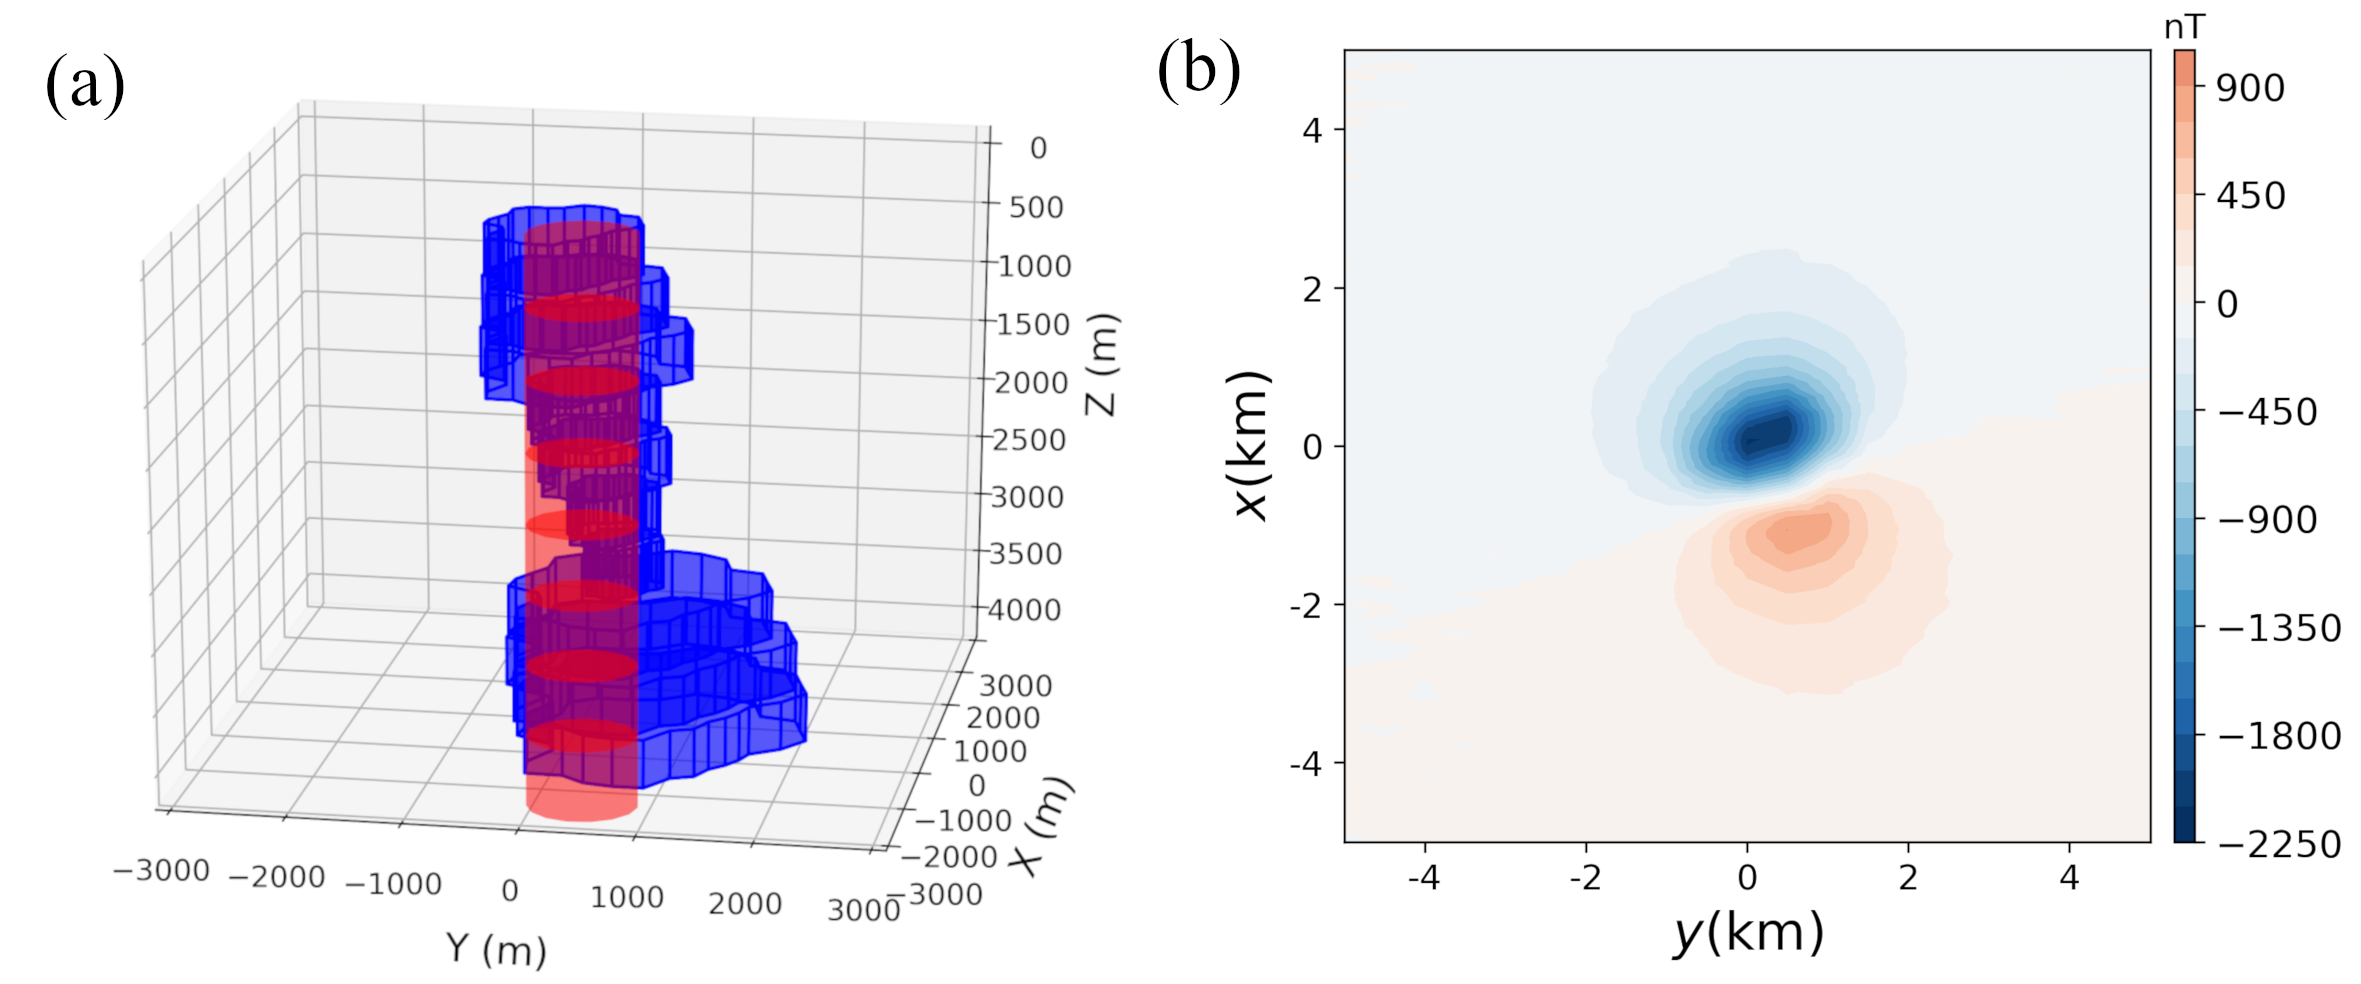
\includegraphics[scale=.75]{figures/complex_3d_ini_data.png}
    \caption{(a) Perspective view of the complex model (blue prisms) with the depth to the top $z_0 = 200$ m and the depth extent $4000$ m and the initial guess (red prisms) for the inversion which is a cylinder with radius $500$ m and depth extent $4800$ m. (b) Synthetic noise-corrupted total-field anomaly produced by the complex model blue prisms in (a). The data was contaminated by a pseudorandom Gaussian noise with mean zero and standard deviation $5$ nT.
}
    \label{fig:complex_model}
\end{figure}

\begin{figure}
    \centering
    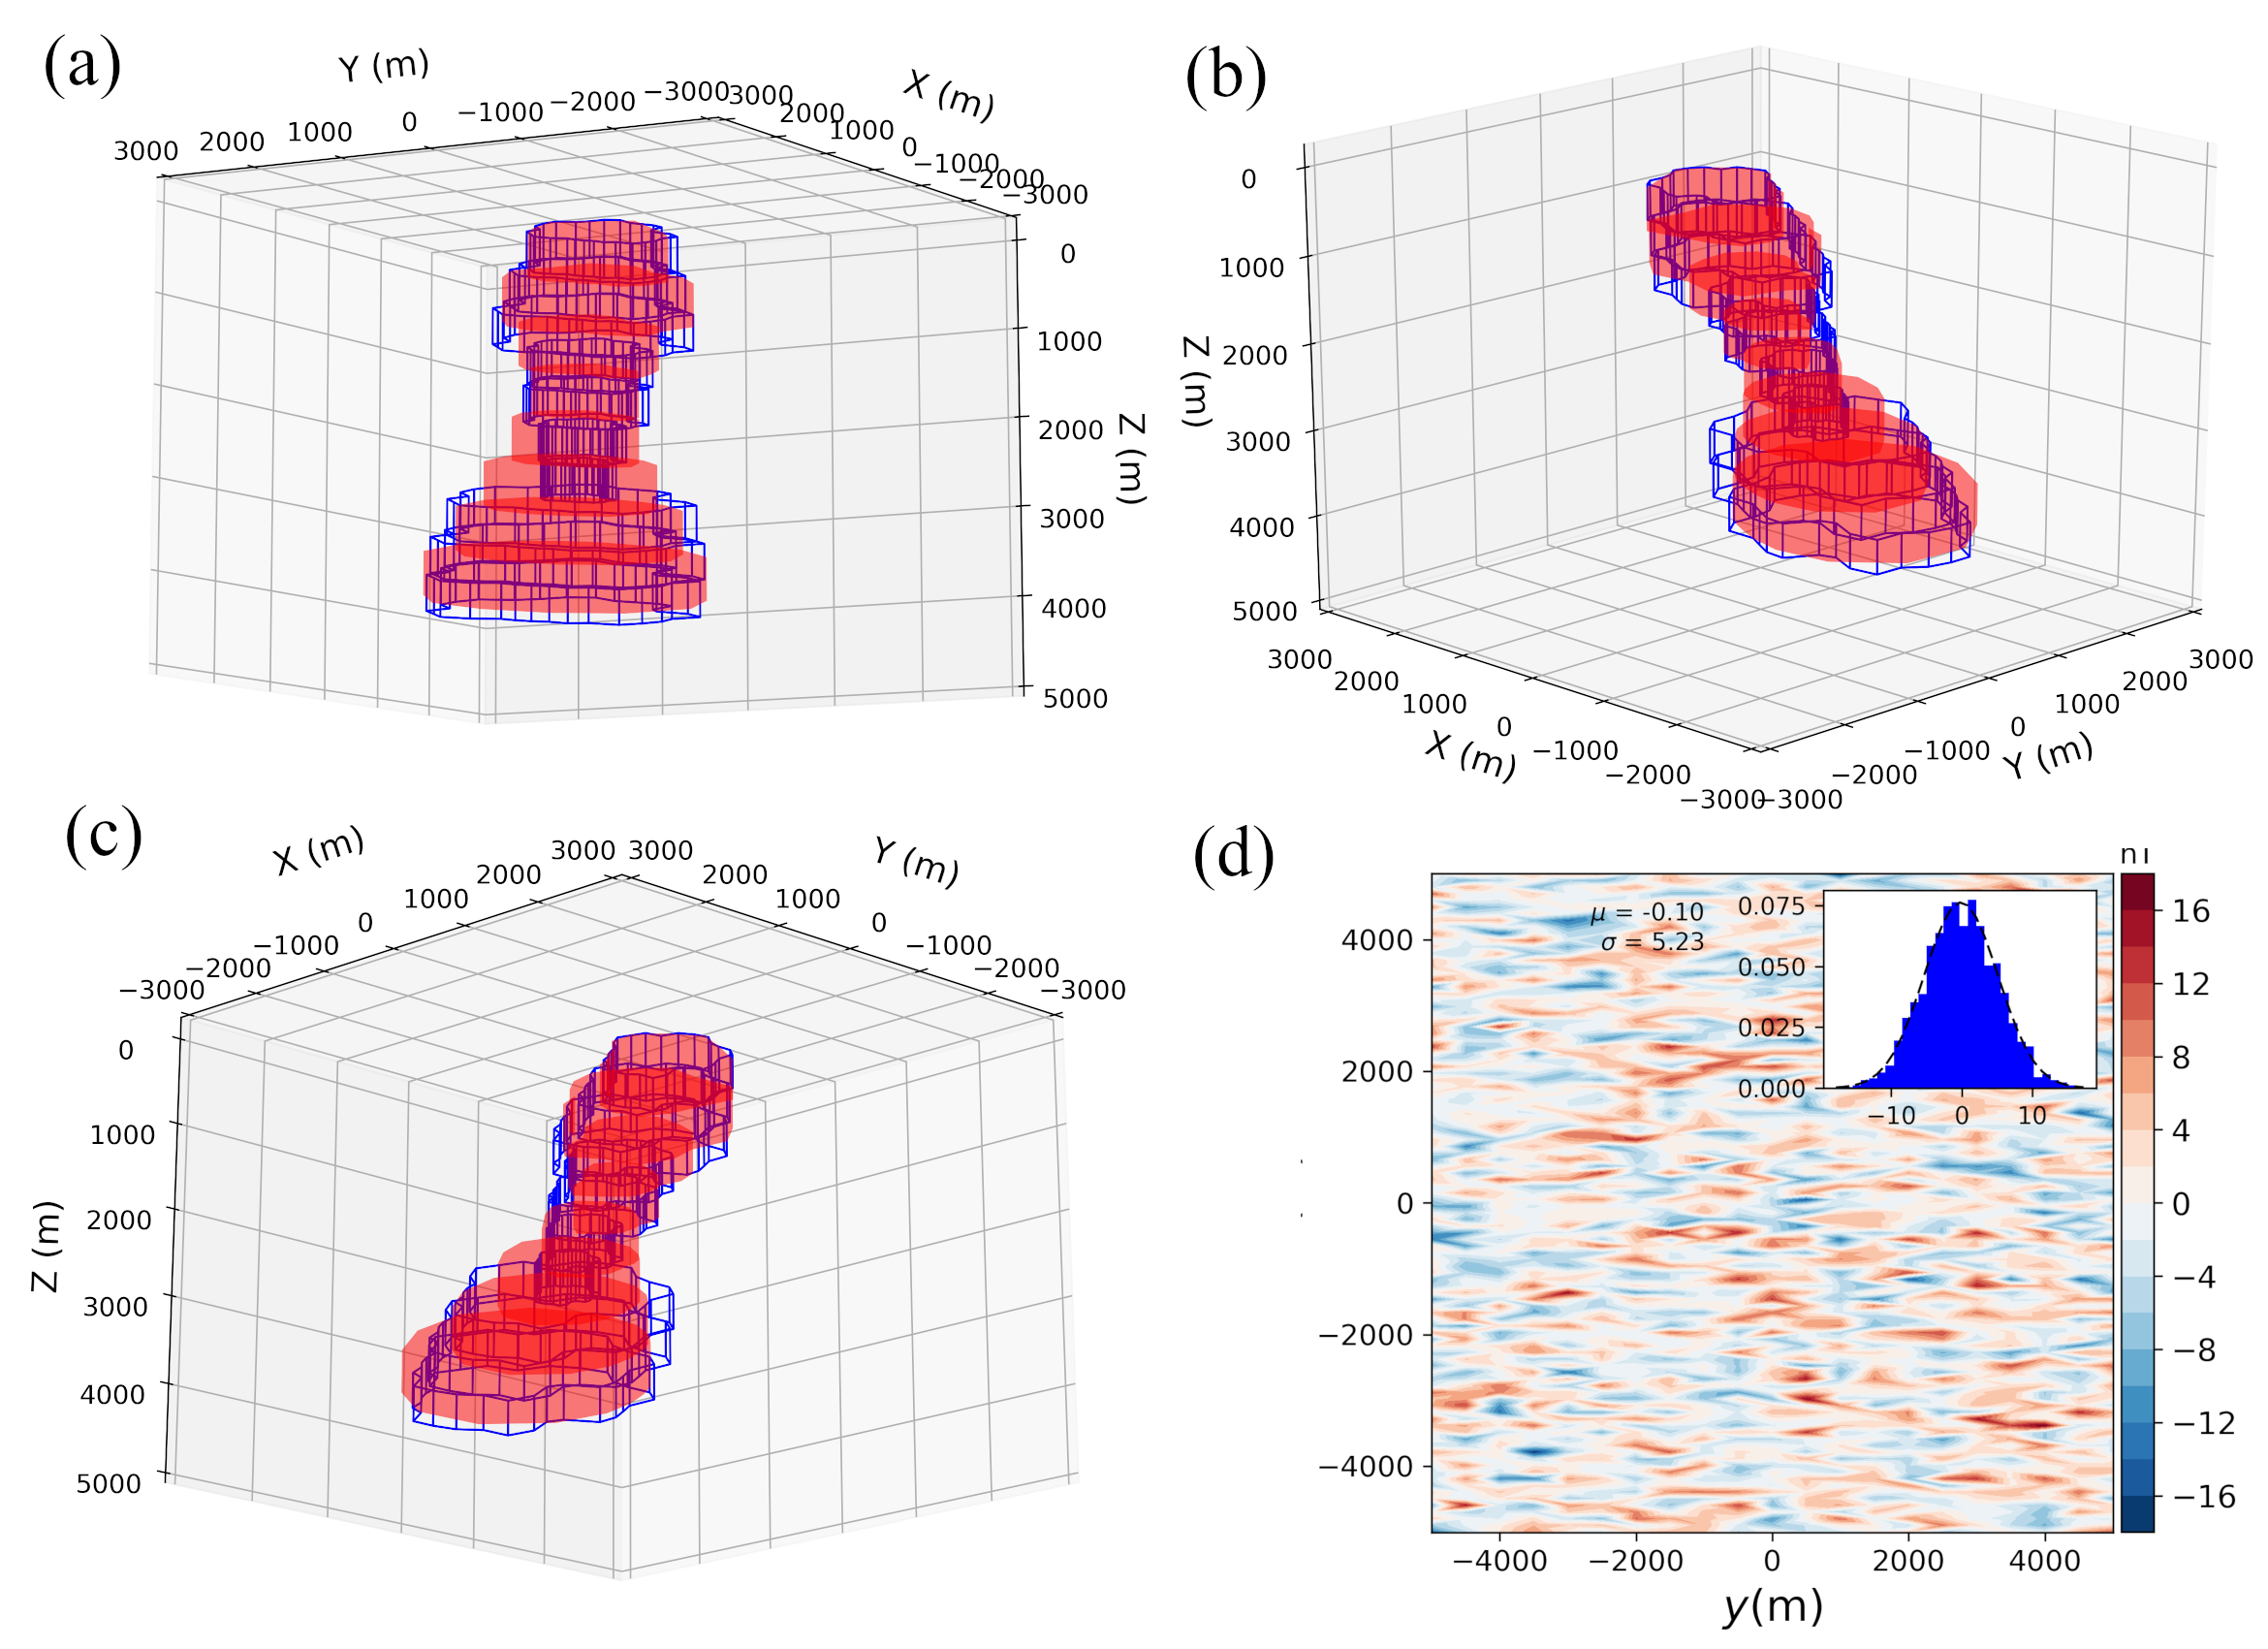
\includegraphics[scale=.75]{figures/complex_estimates_residual.png}
    \caption{Perspective views of the complex model (blue lines) and the estimate (red prisms) in (a), (b) and (c). (d) Residuals defined as the difference between the noisy and the predicted (not shown) total-field anomalies and the histogram of the residuals (inset in d) with mean $\mu=0.1$ nT and standard deviation $\sigma=5.23$ nT. The dashed line on the inset is the Gaussian curve for the residuals.
}
    \label{fig:complex_result}
\end{figure}

\begin{figure}
    \centering
    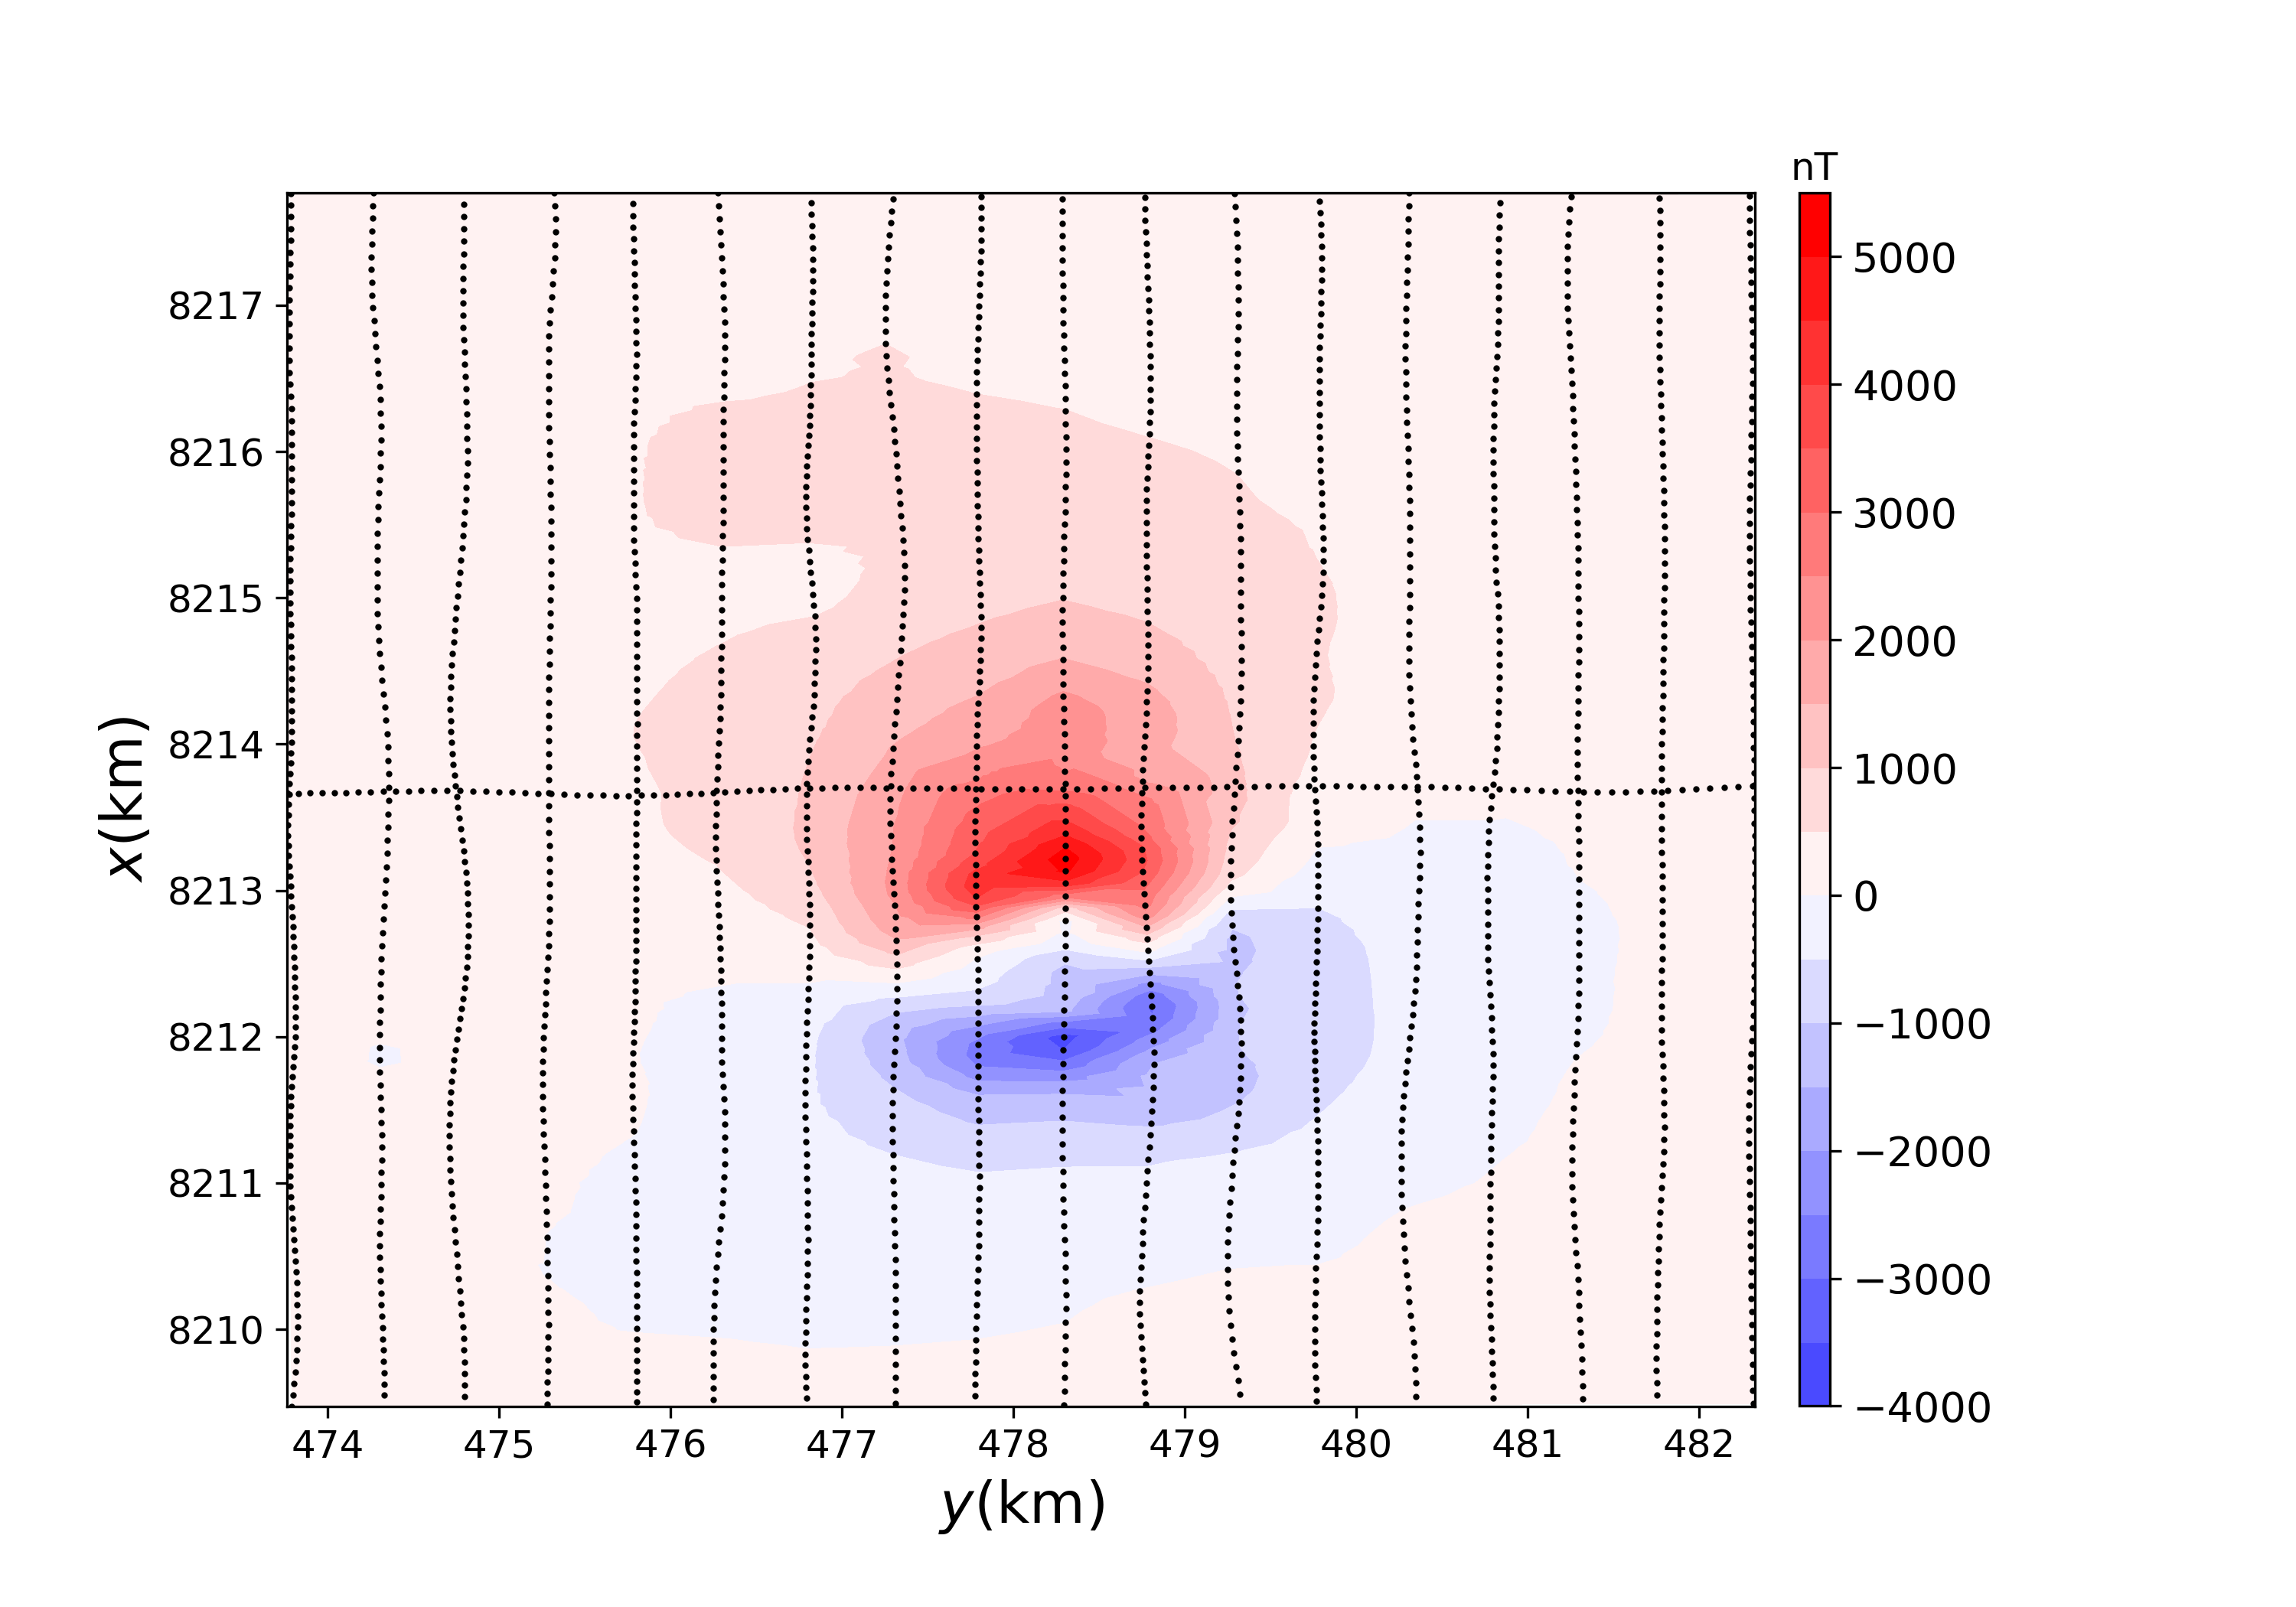
\includegraphics[scale=.5]{figures/diorama_real_data.png}
    \caption{Total-field anomaly of Diorama in GAP. The black dots are the observation points used in this work.
}
    \label{fig:real_data}
\end{figure}

\begin{figure}
    \centering
    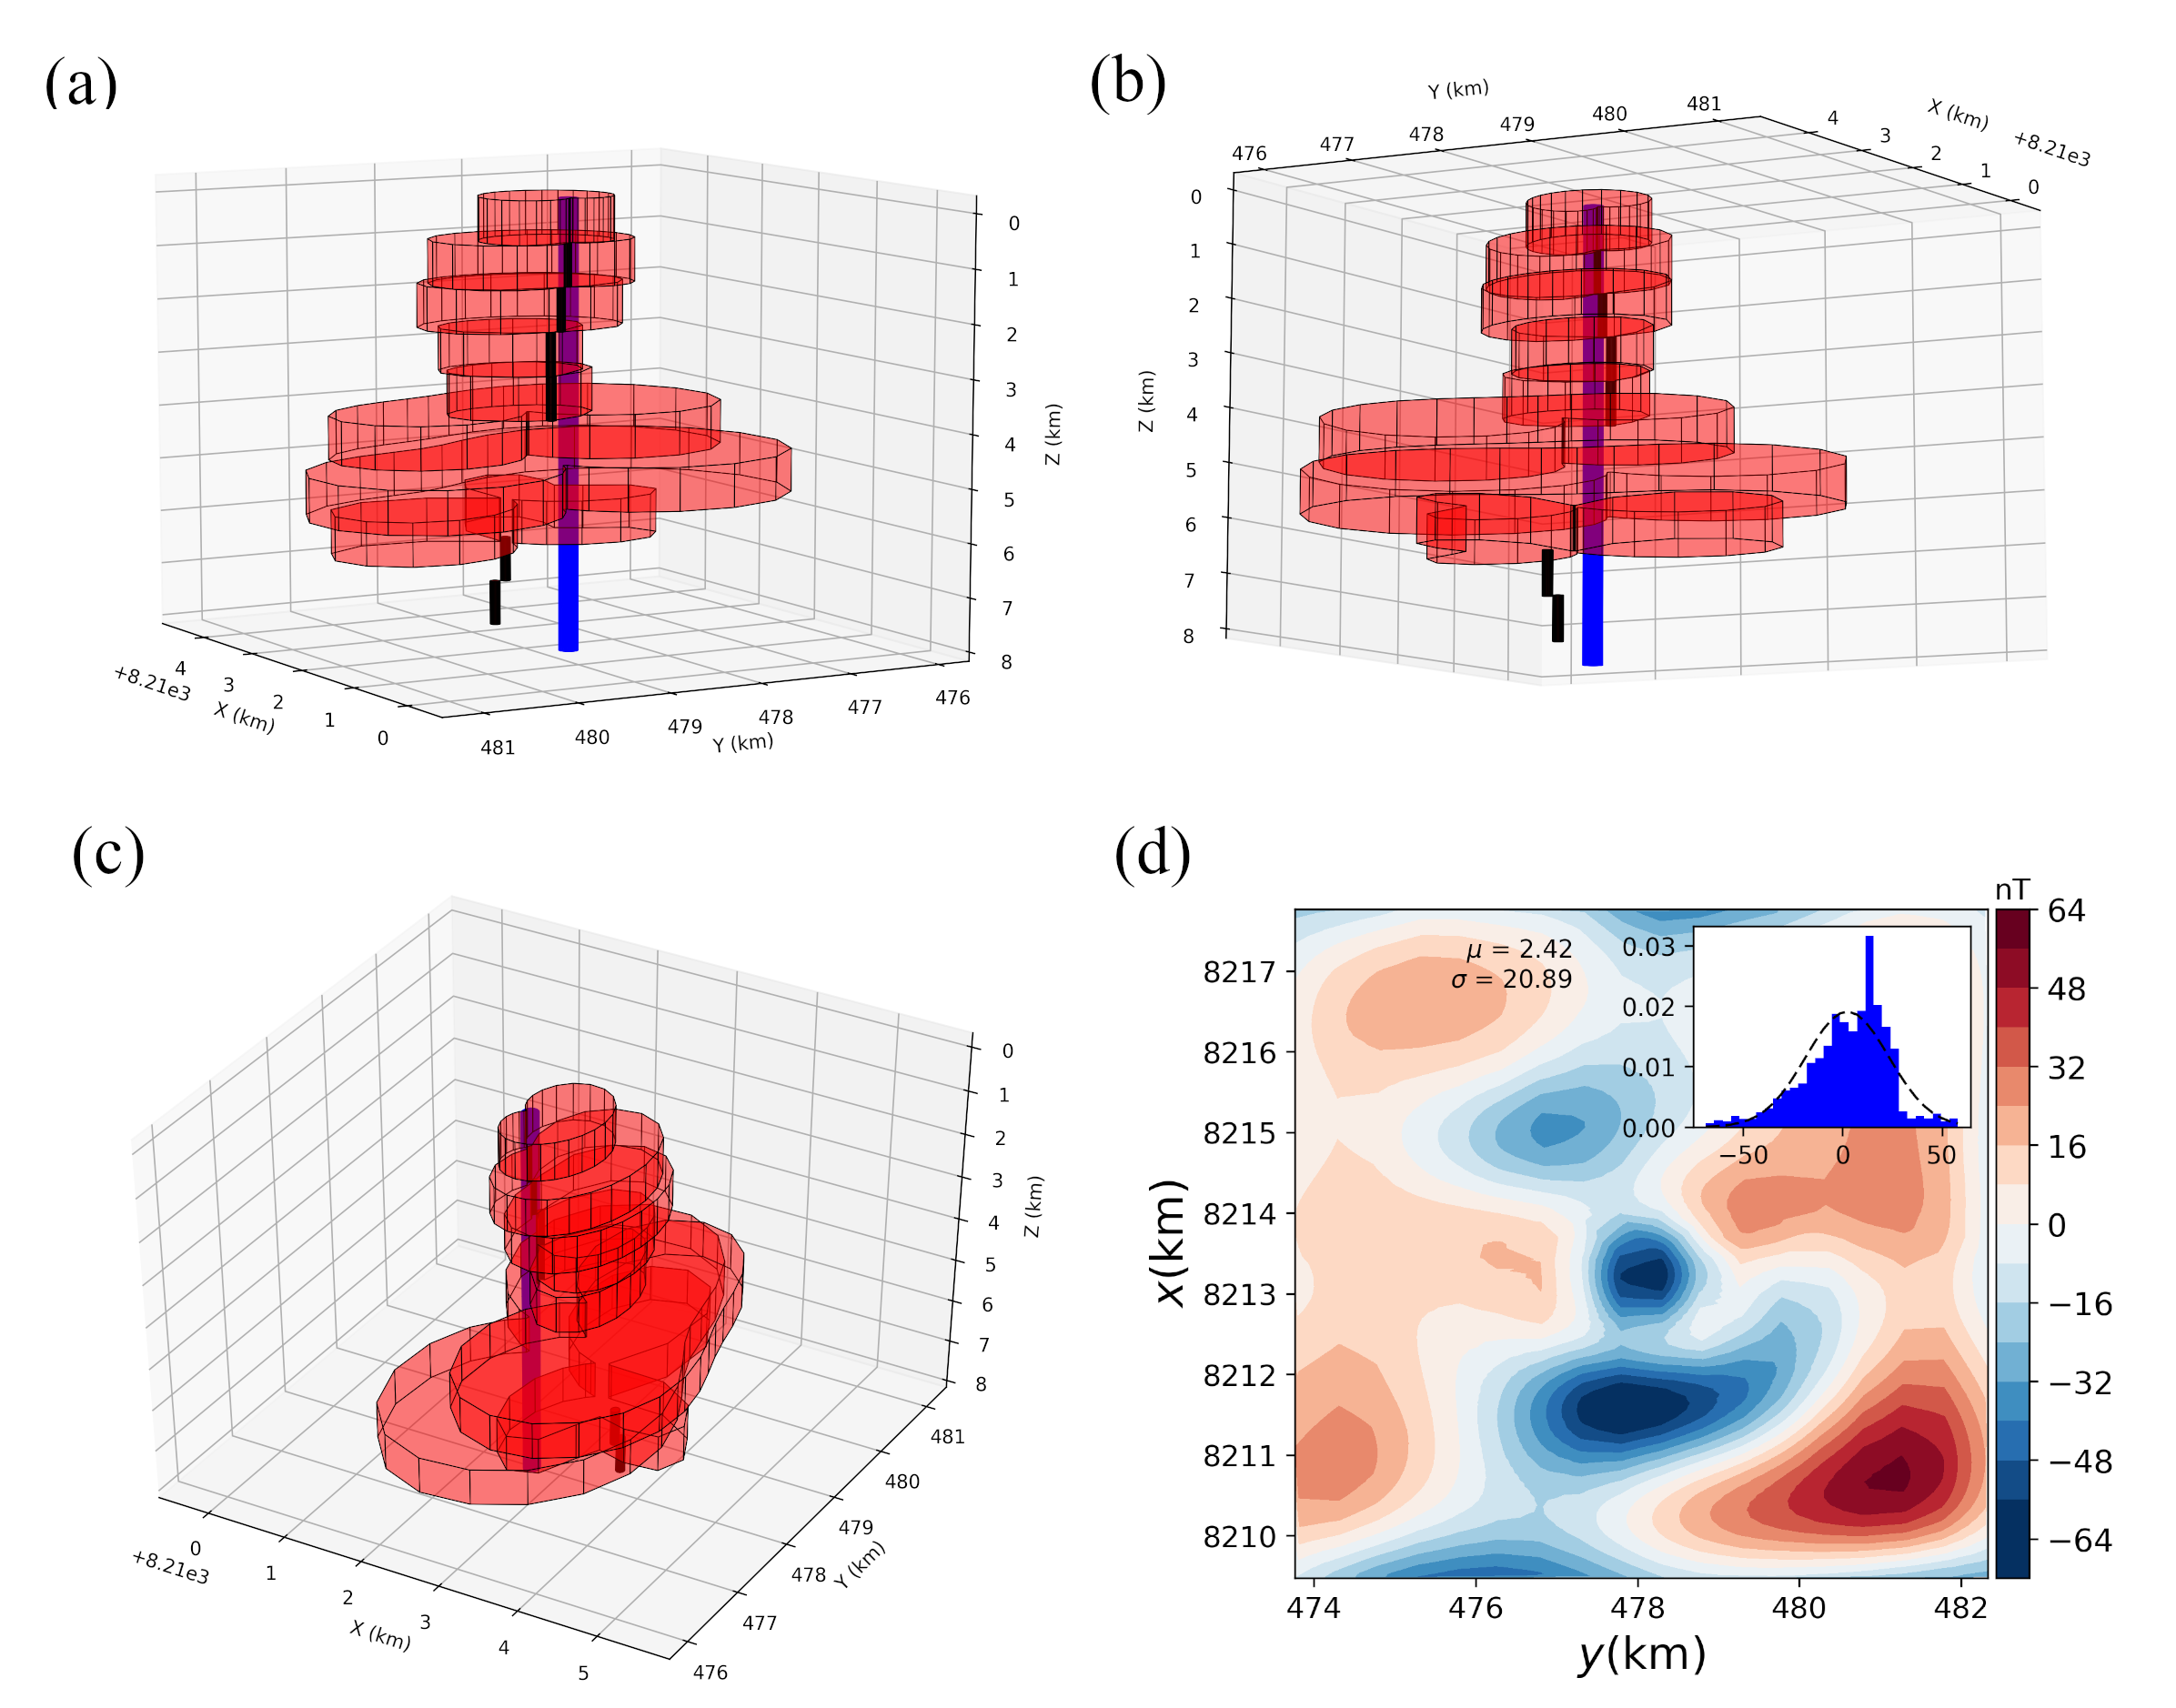
\includegraphics[scale=.75]{figures/real_data_estimates.png}
    \caption{Perspective views of the initial guess (blue cylinder) and the estimated source (red prisms) in (a), (b) and (c). (d) Residuals defined as the difference between the noisy and the predicted (not shown) total-field anomalies and the histogram of the residuals (inset in d) with mean $\mu=2.42$ nT and standard deviation $\sigma=20.89$ nT. The dashed line on the inset is the Gaussian curve for the residuals.
}
    \label{fig:real_result}
\end{figure}